\documentclass[12pt]{amsart}

\addtolength{\hoffset}{-2.25cm}
\addtolength{\textwidth}{4.5cm}
\addtolength{\voffset}{-2.5cm}
\addtolength{\textheight}{5cm}
\setlength{\parskip}{0pt}
\setlength{\parindent}{15pt}
\usepackage{listings}
\usepackage{amsthm}
\usepackage{amsmath}
\usepackage[spanish]{babel}
\usepackage[sort&compress, numbers]{natbib}
\usepackage{amssymb}
\usepackage[utf8]{inputenc}
\usepackage[colorlinks = true, linkcolor = thistle, citecolor = thistle, final]{hyperref}
\usepackage{listings}
\usepackage{ragged2e}
\usepackage{subcaption} 
\usepackage{minted}
\usemintedstyle{borland}
\usepackage{multicol}
\usepackage{listings}
\usepackage{xcolor}
\usepackage{graphicx}
\usepackage[sort&compress, numbers]{natbib}
\usepackage{xcolor}
\usepackage{listings}
\usepackage{ragged2e}
\usepackage{graphicx}
\usepackage[sort&compress, numbers]{natbib}
\usepackage{xcolor}
\usepackage{listings}
\usepackage{ragged2e}
\hypersetup{
    colorlinks=true,
    linkcolor=violet,
    filecolor=violet,     
    urlcolor=violet,
    citecolor=violet,
}
\usepackage{graphicx}
\usepackage[sort&compress, numbers]{natbib}
\usepackage{xcolor}
\usepackage{listings}
\usepackage{ragged2e}

\lstset{style=mystyle}
\usepackage{graphicx}
\usepackage{multicol}
\usepackage{ marvosym }
\newcommand{\ds}{\displaystyle}


\pagestyle{myheadings}

\setlength{\parindent}{0in}
\begin{document}

\pagestyle{empty}



\thispagestyle{empty}

{\scshape Simulación} \hfill {\scshape \Large Tarea 5: Método Monte-Carlo} \hfill  {\scshape 15/Mar/2021}
\author{C. María Montemayor Palos}
\maketitle

\hrule
\hrule
\bigskip


\section{Objetivo}
Examinar y analizar los resultados aplicando el método Monte-Carlo para así estimar el resultado de una integral definida determinando el tamaño de la muestra para la precisión por lugar decimal, comparando el resultado con Wolfram Alpha \cite{wolf} de dos a cinco decimales. Finalmente representando los resultados en un diagrama de violín \cite{dra}.


\section{Metodología}
Para efectos de la tarea se utiliza el programa R versión 4.0.4 \cite{R} para Windows. Se pretende calcular el valor de la integral \eqref{ec1} para la función \eqref{ec2} empleando el método Monte-Carlo y comparar el valor obtenido por Wolfram Alpha de 0.048834.
\begin{equation} 
 \int_{3}^{7} f(x) dx 
\label{ec1}
\
\end{equation}

\begin{equation}
f(x) = \frac{1}{exp(x) + exp(-x)}
\label{ec2}
\end{equation}
La función es posible ya que la función $\displaystyle\int_{-\infty}^{\infty}
  \frac{2}{\pi} f(x) \text{d}x$  es una distribución de probabilidad válida, es decir, la integral de esa función es igual a uno; por esto se pueden crear valores aleatorios basados en esta. Se utilizan estos valores para calcular el área entre los límites de la integral, usando la suma de los valores entre los límites derecho e izquierdo se tendrá el valor aproximado del área, como se muestra en la figura \ref{fig1}.
\begin{figure}[h!]
    \centering 
    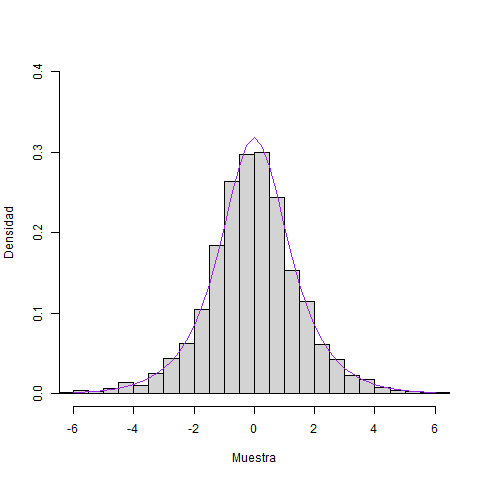
\includegraphics[width=0.4\textwidth]{t5-histograma.png}
    \caption{Histograma de g(x) comparado con g(x).}
    \label{fig1}
\end{figure}
\newpage
Se modifica el código de Schaeffer \cite{dracodigo} para calcular el valor de la integral empleando como números de muestra 50000, 100000, 500000 y 1000000, estableciendo diez réplicas del experimento, posteriormente se comparan los resultados con el valor esperado para comprobar la precisión de los decimales.

\section{Código}
Se establece el número de réplicas del experimento y la variación en el tamaño de las muestras para cada réplica. El código completo se encuentra en el repositorio de Montemayor \cite{mtyor}.
\renewcommand{\listingscaption}{Código}
\begin{listing}[H]
  \begin{minted}[linenos,mathescape,texcl]{clojure}
    n=c(50000,100000,500000,1000000)
    replica=10
    inicio= -6
    final= -inicio
    aum=0.25
    x=seq(inicio,final,aum)
  \end{minted}
  \label{codigo1}
\end{listing}
Se ejecuta la función que calcula la integral guardando así los resultados en el vector \texttt{datos}.
\renewcommand{\listingscaption}{Código}
\begin{listing}[H]
  \begin{minted}[linenos,mathescape,texcl]{clojure}
    for(muestra in n){
        for(r in 1:replica){
         montecarlo = foreach(i = 1:cuantos, .combine=c) %dopar% parte()
        integral = sum(montecarlo) / (cuantos * muestra)
        resultado=((pi / 2) * integral)
        datos <- c(datos,resultado)
        print(resultado)
  }
}
  \end{minted}
  \label{codigo2}
\end{listing}
Se usa la comparación de cadenas de caracteres para comprobar la precisión de los decimales. Posteriormente se convierten los resultados a cadenas de caracteres para comparar y se guarda en el vector \texttt{resultados\_str}.
\renewcommand{\listingscaption}{Código}
\begin{listing}[H]
  \begin{minted}[linenos,mathescape,texcl]{clojure}
    resultados <- c()
    resultados_str <- c()
    res_contadores <- c()

for(i in 1:length(data.matrix(datos))) {
  resultados <- c(resultados,data.matrix(datos)[i])
  resultados_str <- c(resultados_str, strsplit(paste(resultados[i]), split=""))
}
  \end{minted}
  \label{codigo2}
\end{listing}
\newpage
Finalmente se calcula la precisión de los decimales, se comparan y se incrementa la variable \texttt{contador} en uno cada vez que los resultados aciertan en una decimal. El ciclo se detiene cuando no acierta, pues deja de ser preciso en las siguientes decimales.
\renewcommand{\listingscaption}{Código}
\begin{listing}[H]
  \begin{minted}[linenos,mathescape,texcl]{clojure}
for(i in 1:length(resultados)) {
    contador <- 0
    for(muestra in 1:7) {
        b <- (unlist(resultados_str[i])[muestra])
        == (unlist(resultadoEsp_str)[muestra])
        if(b) {
            contador <- contador + 1
        } else {
        break;
        }
    }
    res_contadores <- c(res_contadores,contador-2)
}
  \end{minted}
  \label{codigo2}
\end{listing}

\section{Resultados y discusión}
En la figura \ref{fig2} se muestran los resultados obtenidos a partir del método Monte-Carlo para la estimación de la integral. Se observa que a medida en que aumenta la cantidad de la muestra, el resultado se aproxima mayormente al valor obtenido en Wolfram Alpha. La precisión de los decimales se ve directamente afectada por el tamaño de la muestra, observe cómo en la figura \ref{2a} se logra alcanzar los cinco decimales de precisión en los cuatro tamaños de muestras, con una precisión promedio de cuatro decimales de exactitud como se muestra en la figura \ref{2b}.

\begin{figure}[h!]
\centering
\begin{subfigure}[H]{0.45\linewidth}
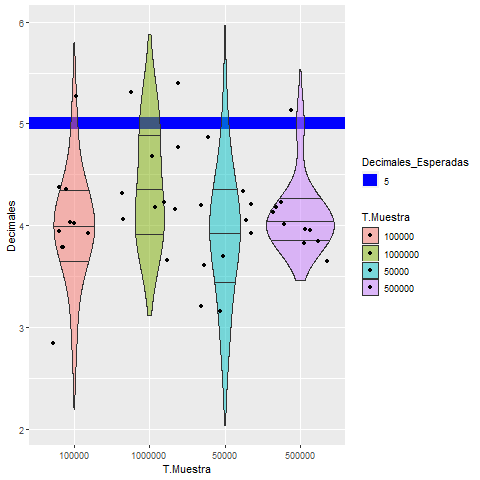
\includegraphics[width=\linewidth]{t5-decimales.png}
\caption{}
\label{2a}
\end{subfigure}
\begin{subfigure}[H]{0.45\linewidth}
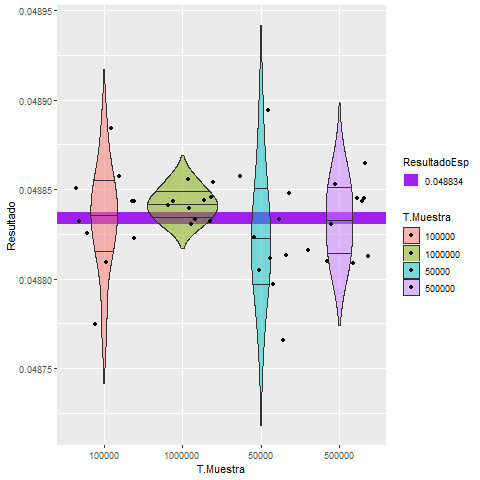
\includegraphics[width=\linewidth]{t5-resultados.png}
\caption{}
\label{2b}
\end{subfigure}
\caption{Comparación de los tamaños de muestra de acuerdo a la precisión de decimales y del valor esperado.}
\label{fig2}
\end{figure}
\newpage
\section{Conclusión}
Si se aumenta el tamaño de las muestras para la estimación de la integral, generará resultados más cercanos al valor real, por lo tanto se recomienda establecer tamaños de muestras más óptimos para tener una buena precisión en los cálculos realizados por el método Monte-Carlo. Así mismo, también es una opción viable replicar el cálculo una cantidad de veces considerable ya que se trabaja con valores aleatorios.
\section{Reto 1}
El objetivo del primer reto consiste en implementar la estimación del valor de $\pi$ de Kurt \cite{kurt} a partir del método Monte-Carlo y determinar la relación matemática entre el número de muestras obtenidas y la precisión obtenida en términos del error absoluto.
Se determinan los tamaños de muestras 100, 1000, 10000, 1000000 y 5000000 considerando como valor $\pi$= 3.141593 con 20 réplicas del experimento.
\begin{figure} [h!]
    \centering
    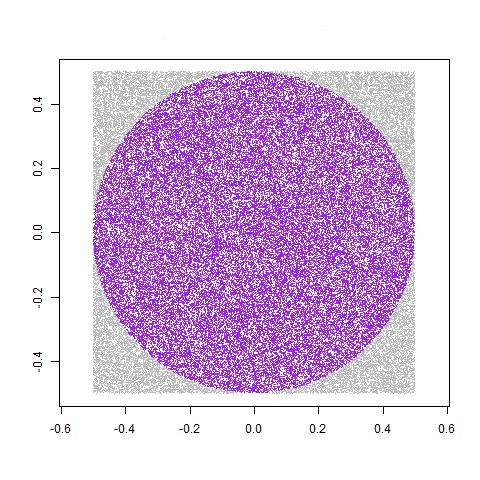
\includegraphics[width=0.6\textwidth]{pi2.jpg}
    \caption{Ilustración del método Monte-Carlo para la aproximación de \pi.}
    \label{fig3}
\end{figure}
Se supone un cuadrado el cual contiene un círculo de radio $r$ en su interior. De esta manera se puede afirmar que el radio
del círculo ($r$) será la mitad de los lados del cuadrado, por lo cual los lados del cuadrado será dos veces el radio del círculo
(2$r$). Para determinar qué área del cuadrado pertenece al círculo se establece la relación en la ecuación \eqref{ec3}.
\begin{equation}
R= \frac{\pi r^2} {4 r^2}
\label{ec3}
\end{equation}
En donde $R$ es la relación del área del cuadrado y el área del círculo, se puede cancelar y despejar $\pi$ para así de esta manera obtener la ecuación \eqref{ec4} que estaremos utilizando para estimar el valor de $\pi$.
\begin{equation}
\pi= 4*R
\label{ec4}
\end{equation}
\newpage
Se estima el valor de $\pi$.
\renewcommand{\listingscaption}{Código}
\begin{listing}[H]
  \begin{minted}[linenos,mathescape,texcl]{clojure}
  calculando <- function() {
  xs <- runif(i,min=-0.5,max=0.5)
  ys <- runif(i,min=-0.5,max=0.5)
  in.circle <- xs^2 + ys^2 <= 0.5^2
  numero <- (sum(in.circle)/i)*4
  return(numero)
}
  \end{minted}
  \label{codigo4}
\end{listing}
Se utiliza el método Monte-Carlo y se obtiene la precisión en términos del error absoluto.
\renewcommand{\listingscaption}{Código}
\begin{listing}[H]
  \begin{minted}[linenos,mathescape,texcl]{clojure}
 for(i in n){
  for(r in 1:replicas){
    montecarlo<-foreach(i = 1:cuantos, .combine=c) %dopar% calculando()
    real <- sum(montecarlo) / cuantos
    Números <- c(Números, real)
    error<-((abs(pi-real))/(pi))*100
    errores<-c(errores,error)
  }
}
  \end{minted}
  \label{codigo5}
\end{listing}
\begin{figure} [h!]
\centering
\begin{subfigure}[b]{0.45\linewidth}
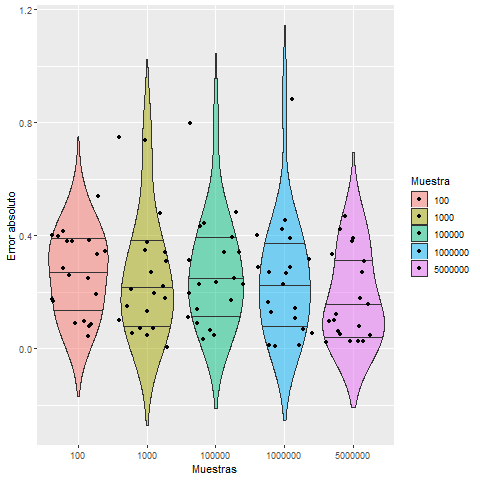
\includegraphics[width=\linewidth]{t5r1-error.png}
\caption{}
\label{a}
\end{subfigure}
\begin{subfigure}[b]{0.45\linewidth}
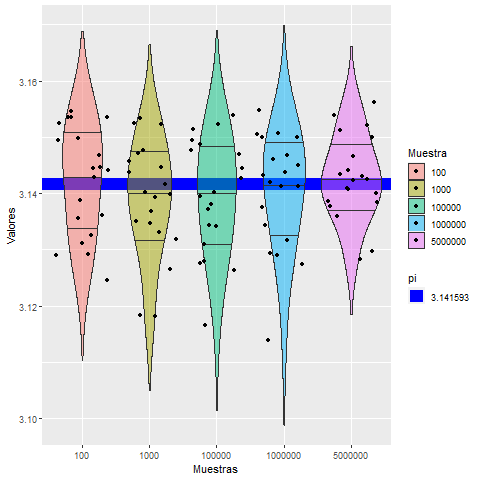
\includegraphics[width=\linewidth]{t5r1-pi.png}
\caption{}
\label{b}
\end{subfigure}
\caption{Comparación de los tamaños de muestra de acuerdo a la precisión obtenida en términos del error absoluto y del valor esperado.}
\label{fig4}
\end{figure}
Se observa en la figura \ref{a} que a medida en que se incrementa los valores de la muestra, menor es el porcentaje de error para la aproximación del valor de $\pi$, entre mayor sea el tamaño de muestra será más acertado el valor para estimar $\pi$. Esto se comprueba
viendo que los valores promedio de todas las replicas y el tamaño de muestra, es decir, los valores generados son muy cercanos al valor esperado de $\pi$ el cual está representado con una línea color azul en la figura \ref{b}. 

\section{Reto 2}
El objetivo del segundo reto es estimar la cantidad necesaria de pintura a utilizar para pintar un mural, aplicando el método Monte-Carlo. Se coomparan los conteos exactos de pixeles con conteos estimados con el muestreo aleatorio.
Se escoge una imagen para el mural, en este caso el logo de Starbucks \cite{star}, en el cual se toma en cuenta que para cada pixel le corresponde $10cm^{2}$ del mural, y que cada litro de pintura rinde $10m^{2}$. Se emplea la librería ``countcolors'' en R \cite{R}, la cual toma en cuenta rangos definidos de colores de pixeles, además genera una imagen en donde sustituye los pixeles a contar por algún otro color de elección para confirmar que corresponda a la región de interés. Se definen los rangos de color y se cuentan exactamente los pixeles por cada rango de color definido.
\renewcommand{\listingscaption}{Código}
\begin{listing}[H]
  \begin{minted}[linenos,mathescape,texcl]{clojure}
white.center = c(1, 1, 1)
green.center=c(0, 0, 0)
png("star-blanco.png")
star.white=countcolors::sphericalRange(star, center = white.center, radius = 0.5,
    color.pixels = FALSE, plotting = TRUE, target.color="cyan")  
blanco=star.white$pixel.count
graphics.off()
png("star-verde.png")
star.green=countcolors::sphericalRange(star, center = green.center, radius = 0.3, 
    color.pixels = FALSE, plotting = TRUE, target.color="blue")  
verde=star.green$pixel.count
graphics.off()
  \end{minted}
  \label{codigo6}
\end{listing}
\begin{figure} [h!]
\centering
\begin{subfigure}[b]{0.27\linewidth}

\includegraphics[width=\linewidth]{star.jpg}
\caption{}
\label{5a}
\end{subfigure}
\begin{subfigure}[b]{0.3\linewidth}

\includegraphics[width=\linewidth]{star-verde.png}
\caption{}
\label{5b}
\end{subfigure}
\begin{subfigure}[b]{0.3\linewidth}

\includegraphics[width=\linewidth]{star-blanco.png}
\caption{}
\label{5c}
\end{subfigure}
\caption{Imagen original del logo de Starbucks y las sustituciones de color de pixeles generadas con countcolors en R.}
\label{fig5}
\end{figure}
\newpage
Para la estimación por el método Monte-Carlo se realiza un muestreo al azar de 10,000 datos y 1,000 repeticiones del experimento, para obtener la media de pixeles correspondientes al color verde, y con ello la estimación de Monte-Carlo. La diferencia del resultado con el total de pixeles de la imagen (307,343) corresponde a la estimación de pixeles de color blanco.
\renewcommand{\listingscaption}{Código}
\begin{listing}[H]
  \begin{minted}[linenos,mathescape,texcl]{clojure}
runs=1000
datos=data.frame()
for(r in 1:length(runs)){
  for(s in 1:10000){
    blue = star[,,3]
    x =sample (blue, runs[r])
    y=sum(x < 0.5)
    print(y)
    datos=rbind(datos,c(s,runs[r],y))
  }
}
  \end{minted}
  \label{codigo7}
\end{listing}
Finalmente se calcula la cantidad de pintura necesaria para un mural de $307m^{2}$ de la imagen.
\renewcommand{\listingscaption}{Código}
\begin{listing}[H]
  \begin{minted}[linenos,mathescape,texcl]{clojure}
pixelesmc=c(mcblanco,montecarloverde)
pixelesmc
pinturamc=pixelesmc*0.001 
pinturamc
  \end{minted}
  \label{codigo7}
\end{listing}
En el cuadro \ref{cua1} se presenta el número de pixeles de color verde y blanco y su respectivo equivalente en litros de pintura para la estimación con números aleatorios y la cuenta exacta. En la figura \ref{fig5} se muestra la figura original del logo de Starbucks, así como las figuras generadas con la librería countcolors, la cual sustituye los pixeles verdes por el color azul \ref{5b}, y los pixeles blancos por el color turquesa \ref{5c}, como confirmación de la cuenta exacta de los pixeles.

\begin{table}[h]
\begin{center}
\caption{Estimación de pixeles y litros de pintura por cada color.}
\label{cua1}
\begin{tabular}{|c c c c c|}
\hline
\textbf{Color}&\multicolumn{2}{c}{\textbf{Monte Carlo}}&\multicolumn{2}{c}{\textbf{Cuenta exacta}}\\
 &Pixeles&Pintura&Pixeles&Pintura\\
\hline
\textbf{Verde}&88,650&88.65 L&76,491&76.49 L\\
\textbf{Blanco}&218,692&218.69 L&230,852&230.85 L\\
\hline
\end{tabular}
\end{center}
\end{table}
En conclusión, se observa que en la aproximación realizada por el método Monte-Carlo se obtuvo una significativa diferencia respecto a la cuenta exacta de pixeles, pero para efectos prácticos si se puede recurrir a este método para darse una idea aproximada de los litros de pintura a usar si se consideran tamaños de murales más chicos.
\clearpage
\bibliography{referencias}
\bibliographystyle{plainnat}


\end{document}
